\documentclass[12pt]{article}
\usepackage[english]{babel}
\usepackage{natbib}
\usepackage{url}
\usepackage[utf8x]{inputenc}
\usepackage{amsmath}
\usepackage{amsfonts}
\usepackage{color}
\usepackage{graphicx}
\graphicspath{{images/}}
\usepackage{parskip}
\usepackage{fancyhdr}
\usepackage{vmargin}
\setmarginsrb{3 cm}{2.5 cm}{3 cm}{2.5 cm}{1 cm}{1.5 cm}{1 cm}{1.5 cm}

\title{Sino: Haymaking challenge}			% Title
\author{Horpynchenko, Dmytro} 								% Author
\date{\today}											% Date

\makeatletter
\let\thetitle\@title
\let\theauthor\@author
\makeatother

\pagestyle{fancy}
\fancyhf{}

\lhead{\thetitle}
\cfoot{\thepage}

\begin{document}

%%%%%%%%%%%%%%%%%%%%%%%%%%%%%%%%%%%%%%%%%%%%%%%%%%%%%%%%%%%%%%%%%%%%%%%%%%%%%%%%%%%%%%%%%

\begin{titlepage}
	\centering
    
\includegraphics[scale = 0.2]{images/sapienza_logo_only.png}\\[1.0 cm]	% University Logo
    \textsc{\LARGE Sapienza University of Rome}\\[2.0 cm]	% University Name
	\textsc{\Large  }\\[0.5 cm]				% Course Code
	\textsc{\Large Interactive Computer Graphics}\\[0.5 cm]				% Course Name
	\rule{\linewidth}{0.2 mm} \\[0.4 cm]
	{ \huge \bfseries \thetitle}\\
	\rule{\linewidth}{0.2 mm} \\[1.5 cm]

	\begin{minipage}{0.4\textwidth}
		\begin{flushleft} \large
			\emph{Author:}\\
			\theauthor
			\end{flushleft}
			\end{minipage}~
			\begin{minipage}{0.4\textwidth}
			\begin{flushright} \large
			\emph{Student Number:} \\
			1807584				% Your Student Number
		\end{flushright}
	\end{minipage}\\[2 cm]


	\vfill

\end{titlepage}

%%%%%%%%%%%%%%%%%%%%%%%%%%%%%%%%%%%%%%%%%%%%%%%%%%%%%%%%%%%%%%%%%%%%%%%%%%%%%%%%%%%%%%%%%

\tableofcontents
\pagebreak

%%%%%%%%%%%%%%%%%%%%%%%%%%%%%%%%%%%%%%%%%%%%%%%%%%%%%%%%%%%%%%%%%%%%%%%%%%%%%%%%%%%%%%%%%
\section{Intro}
As the final project was chosen developing of a browser game that has elements of 3D graphics. 
%Game must be able to run on following list of browsers 
\subsection{Concept}
The world of the game is a field on which hay blocks and obstacles are located. A user is a driver of a vehicle that can move on the field in any direction and collect a hay. In case of collision with the obstacle, vehicle loose all its speed or accelerates in opposite direction in case of high speed. The aim of the game is to collect all hay blocks in defined time period.  Amount of time, hay blocks and obstacles depends on level of difficulty chosen by user. 
\\
The vehicle has 2 controls available:
\begin{itemize}
\item {
Front wheels steering (left and right) using left and right arrow keys. After release of the keys wheels return to their default positions of 0 deg.
}
\item {
Accelerating (forward and backward) using up and down arrow keys accordingly. Release of the keys stop acceleration and leads to deceleration of the vehicle because of the wheel's friction.
}
\end{itemize}
Collecting action is done by colliding with hay block that lead to increase of the score and removing hay item from the field.
\subsection{Name}
The name ``Sino'' comes fron Ukrainian word ``ciho'' - hay \cite{wiki:sino}.


\newpage
\section{Implementation}
\subsection{Overview}
\subsubsection{World}
The world of the game is represented as a simulation of real world with infinite grass field with blue sky around.

\begin{figure}[h!]
\begin{center}
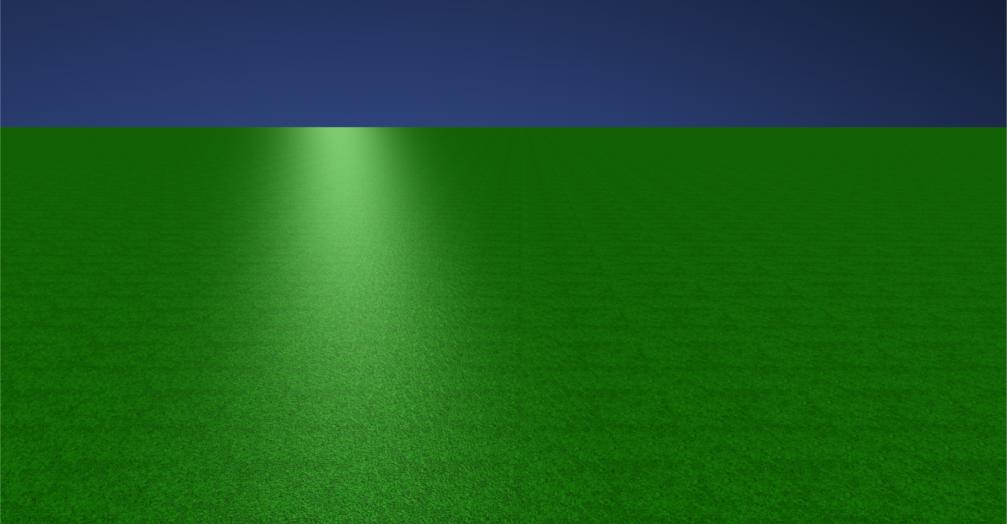
\includegraphics[scale=0.4]{images/env.jpg}
\end{center}
\caption{Game world}
\label{world}
\end{figure}

\subsubsection{Hays and obstacles}
Hays are represented as parallelogram of constant size 1x1x2 with texture of hay (Figure \ref{hay_item}).

\begin{figure}[h!]
\begin{center}
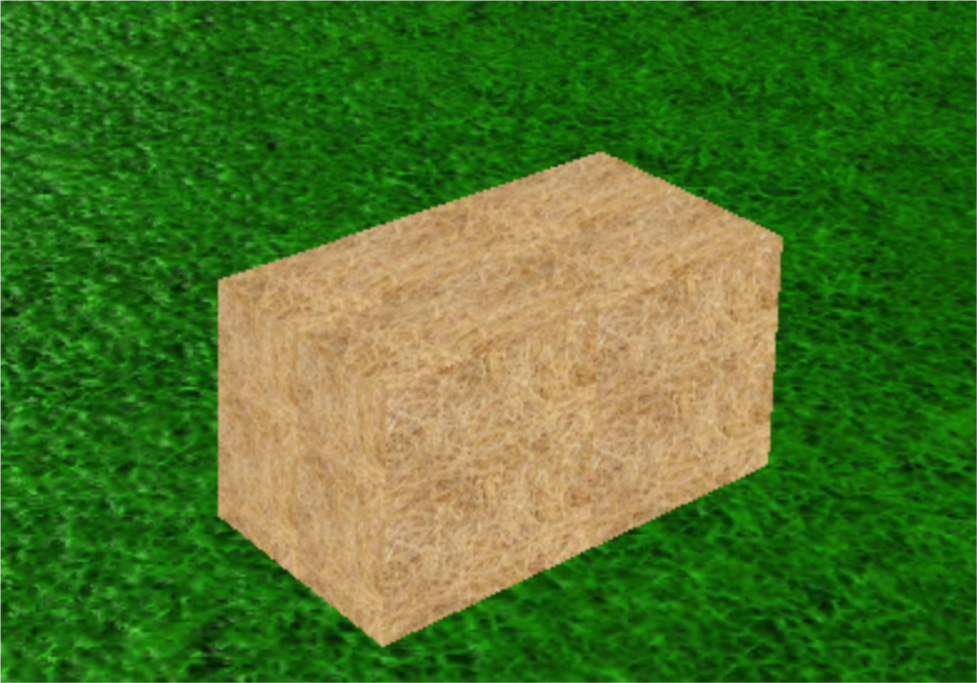
\includegraphics[scale=0.8]{images/hay.png}
\end{center}
\caption{Hay item}
\label{hay_item}
\end{figure}

\par
Obstacles are represented as parallelograms with various sizes. An example of obstacle of size 1x1x4 is showed on Figure \ref{obstacle_item}.

\begin{figure}[h!]
\begin{center}
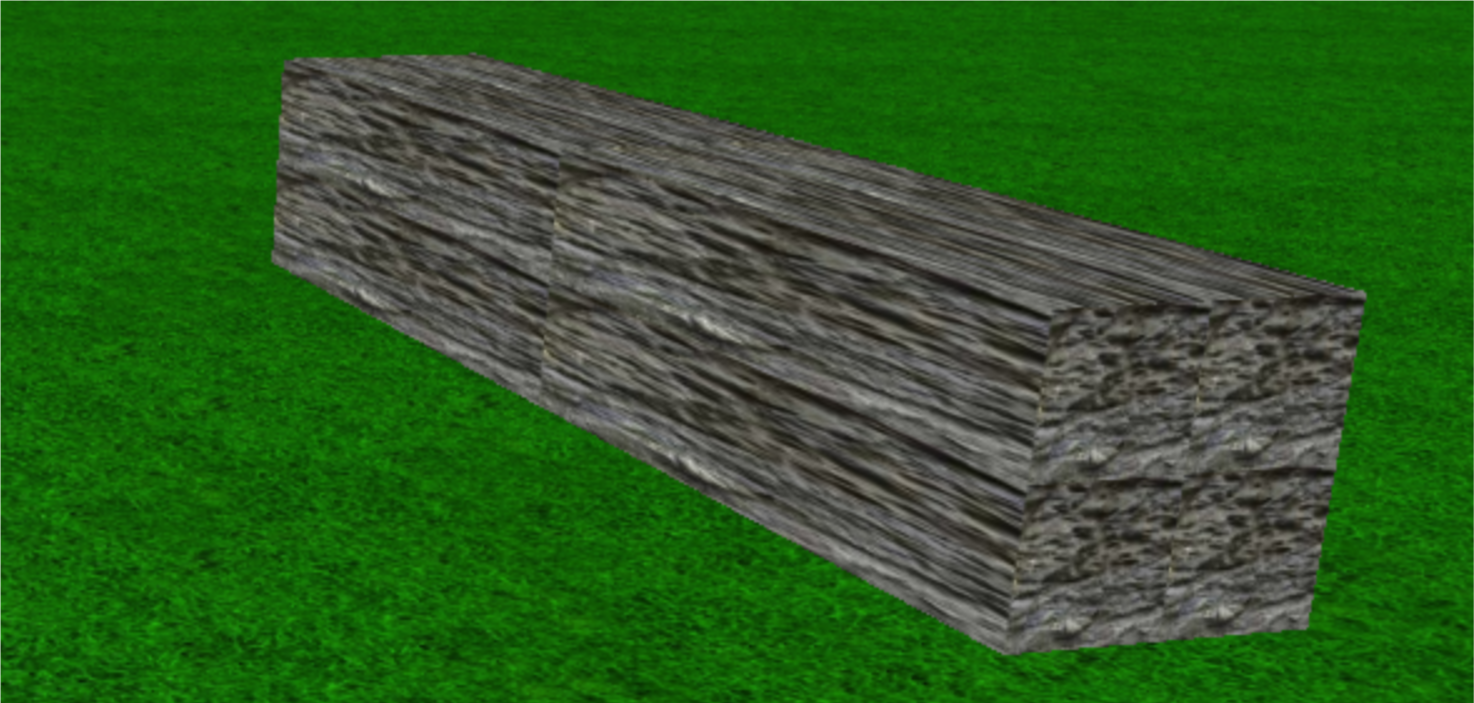
\includegraphics[scale=0.8]{images/obstacle2.png}
\end{center}
\caption{Obstacle item}
\label{obstacle_item}
\end{figure}

\subsubsection{Vehicle}
Vehicle model is a model found on the online marketplace TurboSquid (\url{www.turbosquid.com}). Model represented as tractor vehicle (Figure \ref{tractor1}). For performing an animation 3D model was separated using Blender software into body, front and rear wheels. Every part of the model is exported through Waveform .obj file format for later using during run time. 

\begin{figure}[h!]
\begin{center}
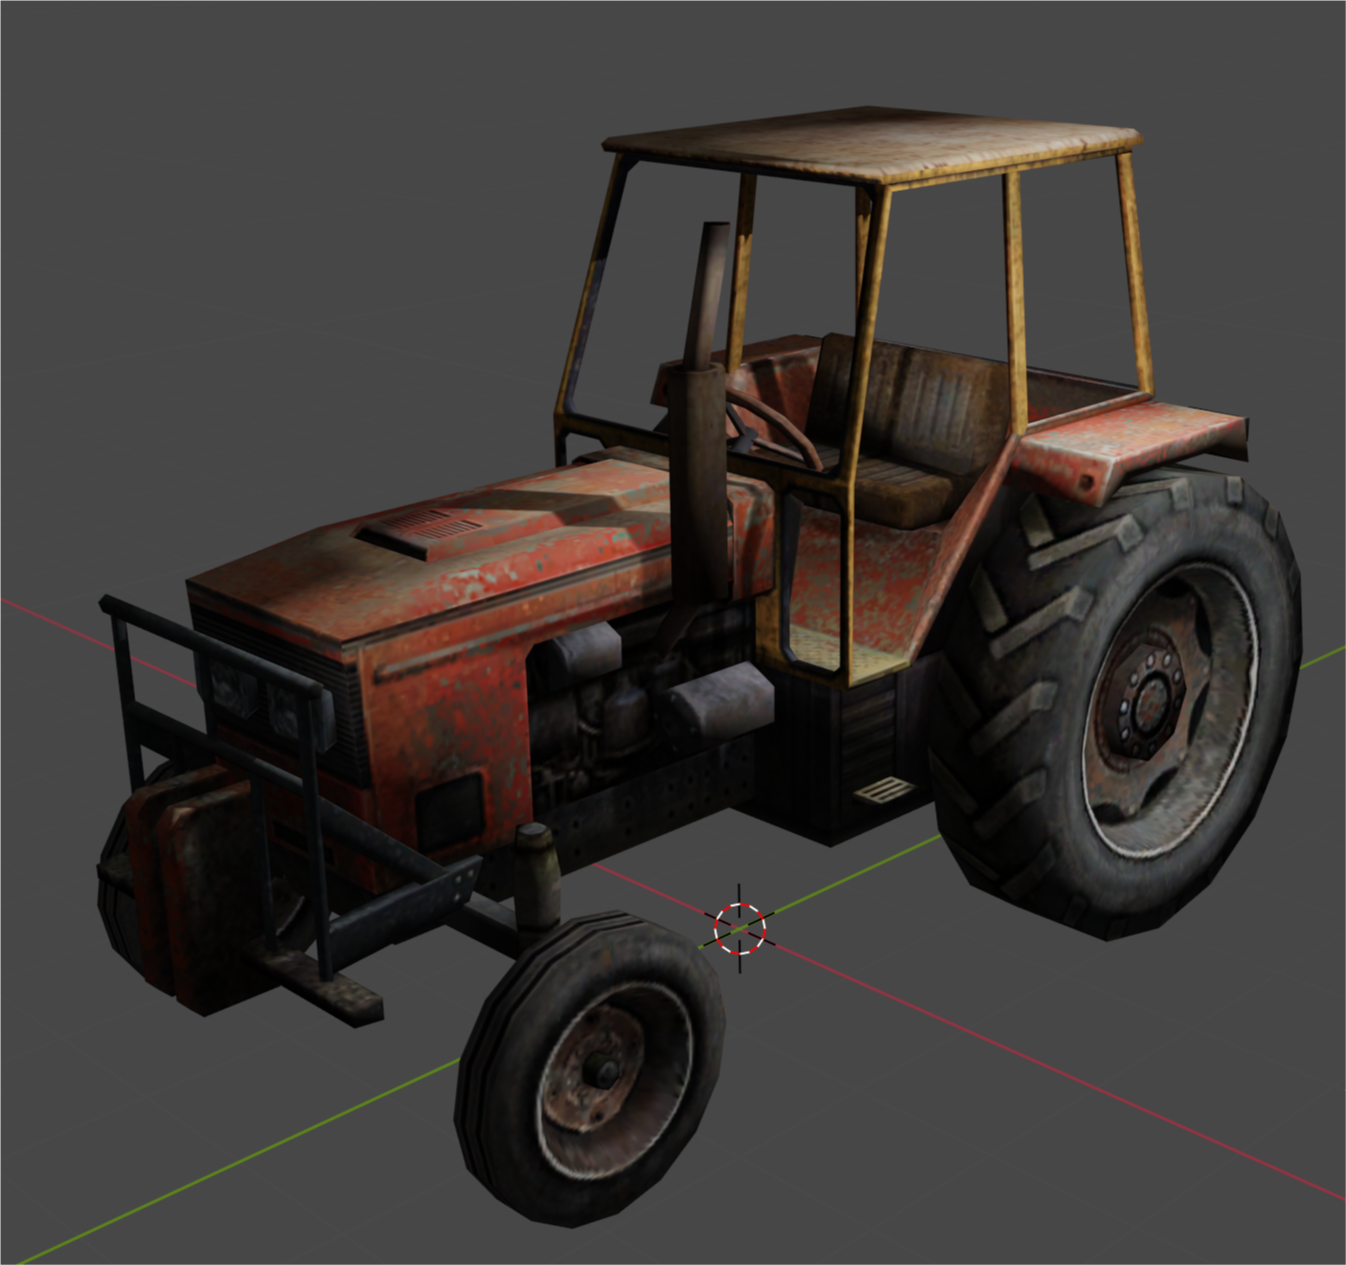
\includegraphics[scale=0.8]{images/tractor_blender.png}
\end{center}
\caption{Tractor model in Blender}
\label{tractor1}
\end{figure}

\subsection{Libraries and Frameworks}
All modern browsers has support of WebGL - a JavaScript API for rendering interactive 2D and 3D graphics with GPU acceleration\citep{wiki:webgl}. But usage of WebGL is quite complicated, requiring writing a lot of boilerplate code, helper functions and hardly maintained code. Thus, in this project THREE.js (\url{https://threejs.org}) open source library was used that offers high-level object-oriented JavaScript API.
\\
Physics emulation libraries like Physi.js or ammo.js weren't used since they are not necessary for game and make big impact on overall performance.
\subsection{HTML}
Hypertext Markup Language (HTML) is the standard markup language for creating web pages and web applications\citep{wiki:html}.
\subsection{CSS}
CSS (Cascading Style Sheets) is a technology that simplify description and declaration of so called ``styles'' or parameters of elements of HTML page\citep{wiki:css}. 
\subsection{JavaScript}
All algorithm part is written in JavaScript and consist if few js files for easy maintenance.
\subsubsection{game.js}
Contains logic initialization part
\subsubsection{core.js}
Contains main components of the code
\subsubsection{items.js}
Maintains initialization of graphical components of the game
\subsubsection{utils.js}
Consist of utility functions that are not depend of the logic and structure of the game.

\newpage
\section{Known Issues}
Testing of final product showed following issues that require additional time to investigation:
\begin{itemize}
\item Performance issues
\item Texture import
\item Bounding Box size increasing depending on rotation of object
\item Adaptation for small screen sizes
\end{itemize}

\newpage
\section{Possible Improvements}
\subsection{Performance}
\subsection{Interface}


\newpage
\bibliographystyle{plain}
\bibliography{biblist}



\end{document}
